\section{waitpid.c}

	Muestre la pantalla de ejecución del programa.

	\begin{center}
		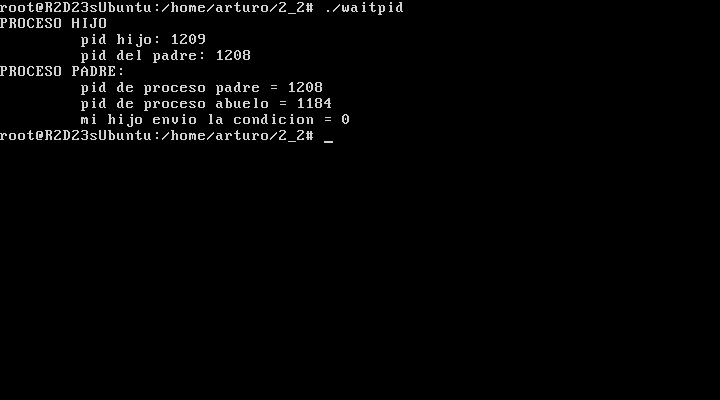
\includegraphics{imagenes/waitpid.png}
	\end{center}

	Describa cuál es el propósito de la siguiente biblioteca:

	\begin{itemize}

		\item sys/wait.h
	\begin{tcolorbox}
	Proporciona lo necesario para trabajar con \textit{waitpid()}.
	\end{tcolorbox}

	\end{itemize}

	Mencione dónde está definida, qué es lo que proporciona de salida y qué argumentos necesita de entrada la función waitpid:

	\begin{itemize}

		\item waitpid
	\begin{tcolorbox}
	Se encuentra definido en sys/wait.h. Espera a que un proceso hijo acabe. 
	\end{tcolorbox}

	\end{itemize}
